\chapter{Pulsating Star - Classical Cepheid}


% Apply a background image to the epigraph region
\begin{tikzpicture}[remember picture, overlay]
  % Place the image (background) in the epigraph area
  \node[anchor=north west, opacity=0.5, scale=1.1,yshift=10cm,xshift=-0.3cm] at (current page.north west) {
    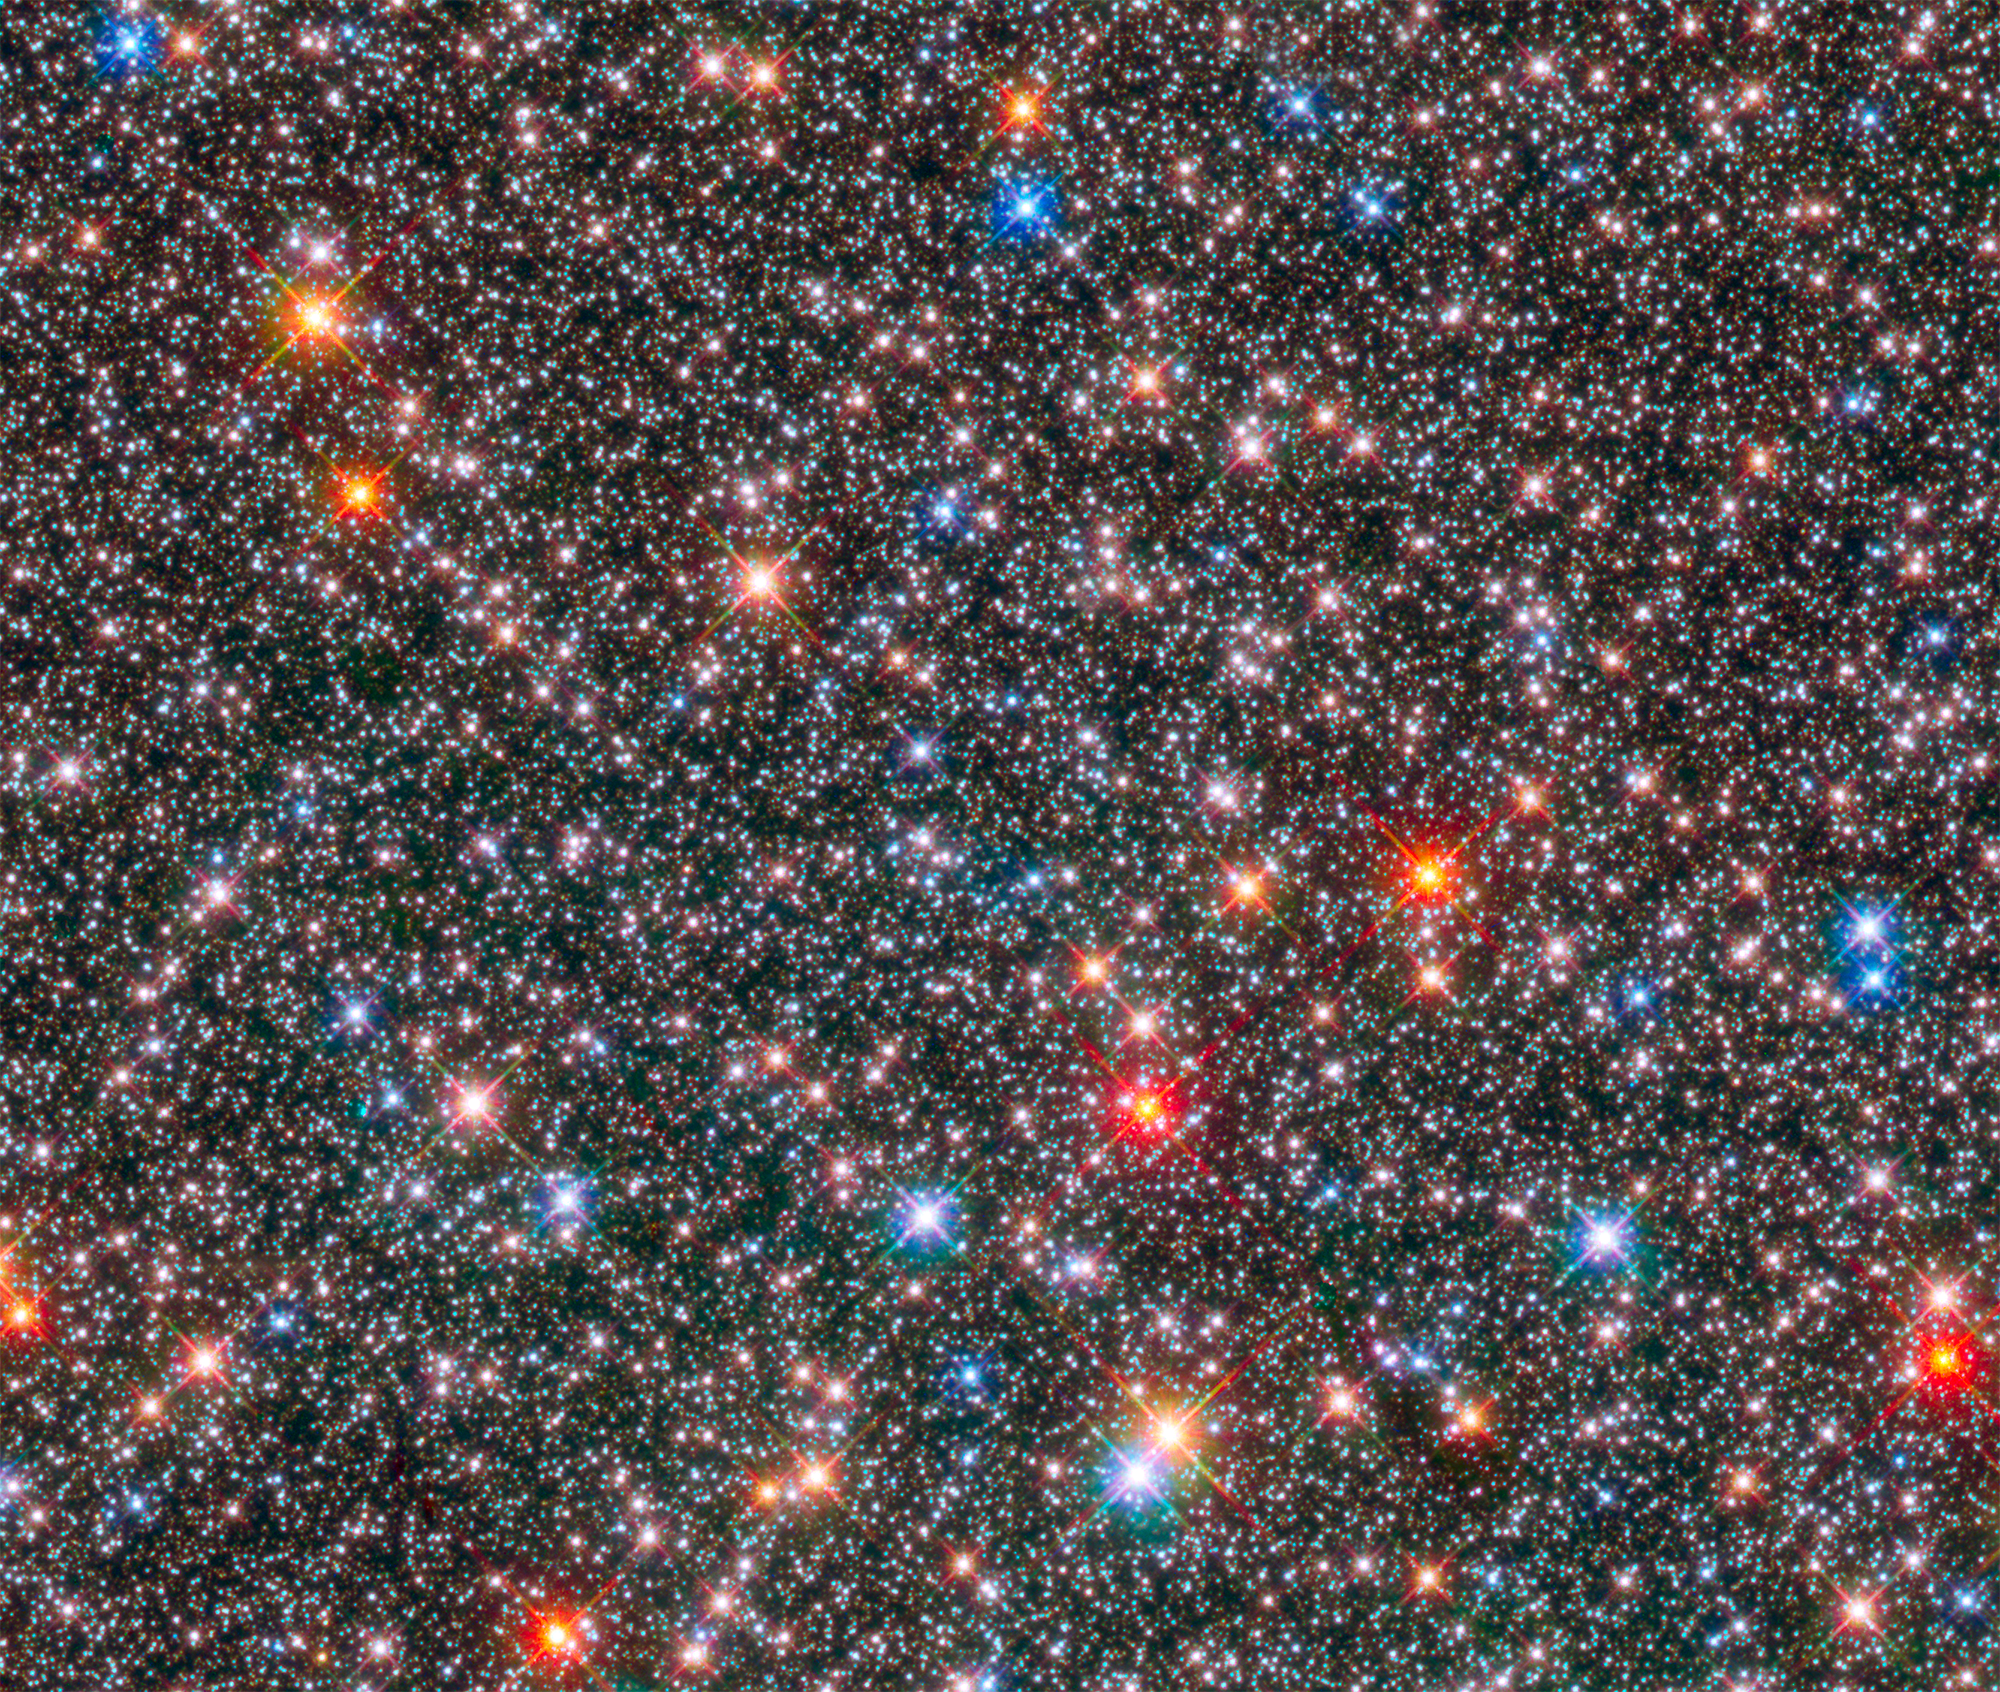
\includegraphics[width=\paperwidth]{../plots/0_images/crowd.png} % Your image path
  };
\end{tikzpicture}



%\epigraph{Who really knows? \\ Who will unfold it? \\ How did this Universe formed?\\ Where does it come from? \\ Gods came after the creation. \\ Then, who really witnessed the origin of this existence?} {Rigved X.129.6}


%https://science.nasa.gov/asset/hubble/milky-way-bulge/



\section{Are all stars the same?}
Seeing the night sky, one can easily spot that stars come in different colors and luminosities, making it easy to infer that not all stars are the same. But what makes them appear different? With the advent of quantum mechanics and spectroscopic observation, this question was answered by explaining the physical processes occurring inside the star, along with changing chemical potential over the different evolutionary phases of the stars. It has been observed that some stars can be thousands of times larger than others—such as red giants and supergiants — while some undergo radial oscillations periodically, like RR Lyrae, Cepheids, and Mira variables. Some stars may form diffuse gaseous systems, such as protostars and planetary nebulae, while others could be the remnants of dead stars, like white dwarfs or neutron stars. These examples represent different phases in the life cycle of a star. This chapter delves into these evolutionary stages, examining how astronomers classify stars, discussing their underlying physics, while focusing particularly on Cepheid variables.

\subsection{Discovery of Variable stars}
The year 1784 is significant in astronomy, as it was when John Goodricke observed the luminosity variation of a star in Cephus consellation - Delta Cephei - challenging the centuries-old belief that the sky is static i.e. all stars being fixed and unchanging \cite{1786john}. Motivated by such a remarkable discovery, the hunt for more variable stars began. Inheriting the name from the first one, variable stars of a similar class were classified as Cepheid variables. Until the twentieth century, it was unclear to astronomers why do Cepheids vary in luminosity. Some suggested a pair of eclipsing binaries \cite{1899pickering} \cite{1903myers} \cite{1914shapley} but spectra shown that it was a single star; others proposed interior effects due to stellar magnetic fields \cite{1908hale} \cite{1914russellvariables} though pulsation was not correlating with magnetic cycle of the star; and some supported the idea of tidal deformation of star's envelope \cite{jeans1917tidal} but light curve did not match with rotation of star. Contribution from Arthur Eddington played a central role in the development of the pulsation theory towards the right path. Mimicking the physics of a reversible heat engine and conceptualized through a valve mechanism (periodically blocking and releasing heat), Eddington formulated the radial pulsation theory of Cepheid variables named as $\kappa$-mechanism \cite{1917eddington}.

Modeling chemical composition and drawing inspiration from Eddington’s valve mechanism for stellar pulsations, Zhevakin, in 1953, proposed that the cyclical ionization of helium envelope drives the radial oscillations observed in Cepheid variables \citep{1963zhevakin}. He modeled a spherical shell consisting of an 85\%–15\% hydrogen–helium mixture (by number of atoms), where helium transitions between the transparent HeI and opaque HeIII states. These ionization transitions modulate the opacity of the stellar envelope, leading to variations in surface brightness and pulsation behavior in Cepheids.

Further developments by S. Chandrasekhar in the hydrodynamic and magnetohydrodynamic stability provided a foundational approach for modelling stellar interior for different masses in various phases \cite{1949chandrasekhar} \cite{1961chandrasekhar}. Utilizing hydrodynamic theory with thermal condition for the stability of Cepheid variable, Cox developed the equation of state of such radially oscillating system \cite{1959cox} . His contribution through non-adiabatic pulsation theory explained $\kappa$- mechanism in detail - how ionized Helium layers changing opacity leads to instability region in Hertzsprung-Russell diagram, also called as instability strip \cite{1968cox} \cite{1980cox}. 

Following in this chapter, a brief summary on the physics of stars and their evolution is discussed. 


\section{Stellar Evolution}
Over the course of their lifetimes, stars vary in size and luminosity depending on their evolutionary phase. Hertzsprung was the first to plot the brightness of a star cluster against its color \cite{1911hertzsprung}, revealing an underlying evolutionary trend. Soon after, Russell independently reached to the similar conclusions \cite{1914russell}. In their honor, this diagram is now called the Hertzsprung-Russell (HR) diagram. For a student of Astrophysics, understanding the color-magnitude is the first step as it play fundamental role in understanding the stellar evolution processes undergoing in different kind of stars.

Stars are classified into three broad categories based on their mass: low-mass, intermediate-mass, and massive stars. These categories follow different evolutionary tracks over their lifespan. As the accumulated matter in a region contracts gravitationally, it reaches stages of threshold densities and temperatures, where different nuclear fusion reactions occur in a natural sequence, starting with hydrogen (1 proton) and progressing to silicon (14 protons + 14 neutrons) which could ultimately fuse to form iron at extreme temperature of 3 billion K . Energy transformation from mass to radiation, heat, neutrino emission, gravitational waves, and other forms is well modeled by quantum physics and gravitational physics, ultimately leads to theory of stellar evolution. In this section, I will briefly summarize the physical processes occurring during the different phases of evolution for each category of star. Following this, we will develop an understanding of the physics behind the pulsations of Cepheid variable stars.

%\begin{figure}[h!]
	\begin{center}
		\includegraphics[width=\textwidth]{../plots/0_images/evol}
	\end{center}
	\caption{Evolutionary cycle for low and high mass star. Low mass stars, like Sun, become a Red Giant when Hydrogen supply to the core stops and fusion takes place in the shell around the core. Afterwards they become a Planetary nebula with a bright core at the center and end their life as a White Dwarf, slowly get faded turning into brown dwarf. Massive stars evolve to Red Supergiant and end their life as Supernova leaving behind either a Neutron star or Black Hole.  [cmglee/NASA Goddard Space Flight Center] }		\label{evolution}
\end{figure}

 
\begin{figure}[h!]
	\centering
	\vspace{-0cm}
	\includegraphics[width = 0.8\textwidth]{../plots/0_images/1992_chiosi}
	\caption{\cite{1992chiosi} HRD}
	\label{1992_chiosi}
\end{figure}
 

\subsection{Formation of Star}

In the vicinity of interstellar nebulae, dispersed gas can collect into dense cloud-like structures called globules, composed mostly of molecular hydrogen (H₂) with trace amounts of heavier elements. Due to the intrinsic mass of the gas, regions of sufficiently high density begin to gravitationally collapse, creating a pressure gradient that slowly raises the core temperature to around 10–30 K. Thermal motion of molecules and radiative cooling initially balance the collapse, stabilizing the temperature for a period. As the collapse continues, the density increases, leading to higher opacity, blocking the radiation causing a gradual rise in temperature. When core temperatures reach roughly 60–100 K, thermal pressure becomes significant enough to temporarily halt the collapse, forming the first hydrostatic core. According to the virial theorem, as mass continues to accumulate, the core temperature rises further.

Once the core temperature reaches approximately 2000 K, molecular hydrogen begins to dissociate, absorbing energy and slowing the temperature rise. This triggers a second, rapid collapse until the core temperature reaches ~10,000–20,000 K, at which point hydrogen becomes fully ionized. The second hydrostatic core is established, supported by the thermal pressure of dense, opaque ionized hydrogen. During this stage, the core’s rotation causes the formation of a rotating accretion disk of infalling material. Gas in the disk follows the trajectories determined by the gravitational potential, often guided along magnetic field lines. Along the polar regions, magnetic pressure dominates over gas pressure, accelerating ionized gas along open field lines and producing highly collimated, supersonic bipolar jets, which manifest observationally as Herbig–Haro objects.

At temperatures ranging from 60 to 100 K, thermal pressure halts the continous gravitational collapse As the protostar continues to accrete mass, it contracts over the Kelvin–Helmholtz timescale, converting gravitational energy into heat. The core temperature steadily rises, eventually reaching $~10^7$ K, sufficient to initiate nuclear fusion.

Nuclear fusion requires that atomic nuclei come sufficiently close for the strong nuclear force to bind them together. However, the positive charges of the nuclei cause Coulomb repulsion, forming the Coulomb barrier. Only at the extreme temperatures and pressures in the protostar’s core do nuclei achieve enough kinetic energy to overcome this barrier. When hydrogen nuclei fuse, primarily via the proton–proton chain, four hydrogen nuclei combine to form one helium nucleus, releasing energy as photons and neutrinos. The onset of sustained hydrogen fusion marks the birth of a star, which enters the main-sequence phase of stellar evolution.

\input{chapters/content/0_3_plot_1934_bethe.tex} 

The first fundamental nuclear reaction in stellar cores is the formation of deuterium (a nucleus containing one proton and one neutron), which occurs at core temperatures of approximately 10–18 million Kelvin. In this process, two protons (hydrogen nuclei) collide at very high velocities, sufficient to overcome the Coulomb barrier and approach within the range of the strong nuclear force (on the order of femtometers). To stabilize the newly forming nucleus, one of the protons undergoes a β⁺ decay (positron emission) process, in which a proton converts into a neutron. At the quark level, this corresponds to an up quark (charge +2/3 e) changing into a down quark (charge –1/3 e), accompanied by the emission of a positron (e⁺) and an electron antineutrino (ν̅ₑ). The resulting proton and neutron then bind together via the strong nuclear force to form a deuterium nucleus. This reaction is the first step in the proton–proton chain, a series of nuclear reactions that release a tremendous amount of energy. The energy output generates radiation pressure, which counteracts the inward pull of gravity, stabilizing the protostar and sustaining its roughly spherical structure over thousands to millions of years.

The first basic nuclear reaction, the formation of Deuterium (nucleus containing one proton and one neutron), requires a temperature of 10 - 18 million Kelvin. In this senario, two protoniums (hydrogen ions) collide with each other at a very high velocity, surpassing the Coulomb barrier and entering to field of strong nuclear force at femto scale. To stablise the new configuration, one of the proton changes its up quark (+1/3) to down quark (-2/3), releasing positron and an electron antineutrino, to converts into a neutron. This process is called as $\beta^{+}$ decay process. Both elementary particles, proton and neutron, stick together to form nucleus of Deuturium. Series of such nuclear reactions release an immense amount of energy radiating outwards. Radiation pressure counter balances the continous gravitation collapse of the matter, sustaining the spherical structure of the protostar for thousand to million years. The energy released from fusion reactions in stars calculated by Bethe and published under title - 'Energy production in stars'\citep{1939bethe}. At the heart of these calculation, Einstein's famous equality $E = \Delta m c^2$ underlies which tranforms mass into energy. Here, c is the speed of light and $\Delta m$ is the difference between the mass of reactants and products of the fusion reactions. 


\begin{notebox}[sharp corners, width=\textwidth]{Nuclear Fusion Reactions in Main Sequence Star}

{\small Accumulation of Deuterium opens possibility for fusing with one more proton to form Helion (2 protons and 1 neutron). Rising temperature fuses two Helion atoms to form Helium (2 protons and 2 neutrons) and emits two Hydrogen atoms. This series of reactions from Hydrogen to Helium is called p-p chain (pp I branch) reaction. Other rarer reactions can also occur, for instance, pp II branch when Helion fuses with Helium to form Beryllium (4 protons and 3 neutrons). Then either Beryllium decays to Lithium (3 protons and 4 neutron), Lithium fuses with proton and breakdown into two Helium atoms. Otherwise, in pp III branch, Beryllium fuses with proton to form Boron (4 proton and 4 neuton) which is unstable and breaks down into two Helium. The most rare case is pp IV branch, when Helion captures a proton and form Helium. 
%Source: F. Reines, Ann. Rev. Nucl. Sci. 10 (1960) 1-26}
}

Proton-Proton Reactions: Efficient for 1 $M_0$ star's core. \\

\hspace{1cm} Branch I: 83.30\% Helium production, at 10-18 MK


\begin{center}
	\ce{^1H ->[p][e+,$\nu_e$]^2D ->[^1H][ $\gamma$ ]  ^3He ->[^3He][2 ^1^H] ^4He } 	
\end{center}
%\vspace{-3mm}

\hspace{5.6cm} 0.42 \hspace{0.7cm} 5.49 \hspace{0.7cm} 12.85  \hfill (Energy release in MeV)

\hspace{1cm} Branch II: 16.70 \% Helium production, at 18-25 MK

\begin{center}
	\ce{^4He ->[He][$\gamma$]^7Be ->[e-][ $\nu_e$]  ^7Li ->[H] 2 ^4He }	
\end{center}
\vspace{-2mm}
	\hspace{5.6cm} 1.59 \hspace{0.6cm} 0.861 \hspace{0.3cm} 17.35 \hspace{0.9cm} \hfill (Energy release in MeV)
	\vspace{1mm}

\hspace{1cm} Branch III: 0.12\% Helium production, above 25 MK

\begin{center}
	\ce{^4He ->[He][$\gamma$]^7Be ->[H][ $\gamma$]  ^8B ->[][e+,$\nu$_e] ^8Be -> 2^4He }	
\end{center}
\vspace{-2mm}
	\hspace{4.9cm} 1.59 \hspace{0.6cm} 5.59 \hspace{1.7cm}     23.29   \hfill (Energy release in MeV)


\hspace{1cm} Branch IV: 0.00002\% Helium generation in Sun 

\begin{center}
	\ce{^3He ->[H][e+,$\nu$_e] ^4He}	
\end{center}
	\hspace{7.1cm} 19.795 \hspace{0.3cm}  \hfill (Energy release in MeV)
	
{ \small All these four branches are called pp chain reaction.}
\end{notebox}


The fusion of elements releases vast amounts of heat, radiation and neutrino flux. A star's evolution depends primarily on its initial mass. Massive stars experience stronger gravitational pressure, higher core temperatures, and faster fusion rates, causing them to burn through their fuel more quickly and live shorter lives compared to lower-mass stars. Stars progress through several phases during their evolution, driven by their mass, as shown in Figure \ref{evolution}.


\vspace{1cm}


\subsection{Main sequence star and Turn-off point}



The color of the star gives a rough idea about the surface temperature as well as evolutionary phase of the star. Newly born stars are rich in Hydrogen and fuse it rigorously resulting very high surface temperature making it appear bluer. After millions of years, helium as byproduct accumulates at the core which blocks the supply of Hydrogen and reduces the rate of fusion due to which star cools down and turn yellowish. It is worth to say that, high mass stars exert high pressure at core and burn its fuel quickly as compare to low mass stars. Where lifespan of a high mass star (8-10 $M_\odot$ ) lies around 10-15 million years, for low mass star it can be 15-20 billion years. In its life journey, any star spends most of the time in Main Sequence phase.

\begin{wrapfigure}{r}{0.4\textwidth}
	\centering
	\vspace{-0.7cm}
	% include first image
	\includegraphics[width=\linewidth]{../plots/0_images/Evo2.png}  
	\label{isochrone}
	%\begin{center}
	\caption{Isochrones of stars with different masses depicting their evolutionary traids.  Source: Universe (VIII edition) by Roger A. Freedman \& William J. Kaufmann III}
\end{wrapfigure} 




For the case, when the initial mass of star remained under half of solar mass, after a few billion years, enough Helium get depleted at the core which blocks the hydrogen supply, ultimately reducing the rate of fusion reaction. Star gets cooler with time, finally become redder then a brown dwarf and its life as a black dwarf after trillions of year. Such star never leaves the main sequence but only changes its spectral type as it evolves. For star of one solar mass, when Helium core forms which reduces the rate of fusion reaction, the gravitation pull begins to contract the core and core's temperature increases again. With higher temperature, Hydrogen begins to fuse around the Helium core in a shell, making the star move away from the main sequence and marks the turn-off point in the HR diagram. 

\subsection{Red Giant Star and Helium Flash}
Shell burning Hydrogen generates even more energy than core burning phases. Released energy pushes the envelope of matter outwards which expands the surface of the star enormously and it becomes a giant. With increased surface area and shell H-burning, luminosity of the star increases by the order 3 to 4, however, due to expansion, surface of the star cools down making it red in color. This physical characteristics gives it name - Red Giant. Further accumulation of Helium at the core due to H-shell burning continuous. Star having mass more than 3 solar mass, gradually star helium burning at the core, however stars with mass between 0.3 to 3 solar mass attain Helium fusion spontaneously, called as Helium Flash. For the latter case, central region of the core becomes incompressible but the rest of core still collapses causing further rise in temperature at center, but not sufficiently enough that helium could fuse, so the central core takes the form of degenerate matter to balance the gravitation collapse. 

Around 300 million K, the degenerate matter spontaneously fuses into heavier elements, Carbon and Oxygen, by triple alpha process leaving behind a flash of high energy which rises the temperature exponentially high. Degenerate matter fuses rapidly rising the temperature even higher which accelerate the reaction rate. This thermal runaway reaction increases the energy production of the star to 100 billion times for a very short time, which is comparable to entire galaxy's energy output. Eventually thermal pressure becomes dominant and the core expands. This phase in HR diagram can be observed as the tip of the red gaint branch on the right-upper side for intermidiate mass (0.4 to 3 solar mass). Just after this state, star rearranges its structure rapidly and attain an equilibrium state with a lower luminosity but higher temperature than before. This spontaneous process shifts the star from red gaint branch to horizontal branch while leaving a discontnuity in between the two regions in HR diagram. \footnote{Kristen. B. W. McQuinn et al 2019 ApJ 880 63}    

\subsection{Horizontal branch and Variable stars}

While evolving through horizontal branch, stars fuse Helium at the core and Hydrogen in a shell. Moving towards right side, star enters to the blue edge of instability strip of HR diagram where it experience a dynamic equilibrium between gravitational contraction of outer envelope and its thermal expansion due to energy generation from internal processes. This translated as a radial oscillatory motion of the surface, giving birth to a new category of stars called variable stars. In 1784, John Goodricke had discovered a variable star, $\delta$ Cephei, in Cepheus constellation and named the star as $\delta$ Cephei. After the discovery of a few more variable stars, the family of $\delta$ Cephei type stars called as Cepheid stars. 

Initially, it was assumed that the periodic variation of luminosity arising because the star is a member of eclipsing binary system. In 1917, Arthur Eddington rejected the prior theory and gave a clever explanation behind the radial pulsation of star by purposing a valve mechanism. His purposed mechanism known as Kappa mechanism as kappa stand for coefficient of absorption of stellar material. After excessive burn of hydrogen, helium becomes the next abundant element on the surface. Due to high temperature at the compressed state of Cepheid star, Helium releases its both electrons and get ionized \ce{He^{2+}}. Opaque \ce{He^{2+}} blocks the outcoming radiation making the star appear dimmer. The radiant energy develops a pressure and expands the star's surface. The expansion increases the surface area illuminating the star. Expansion also cools down the surface so the ionized Helium captures the free electrons and back to its ground state \ce{He}. Neutral Helium is a transparent gas consequently, all the trapped radiation releases making the star even more luminous. As the radiation pressure decreases, the stellar surface begin to collapse again due to gravitational pull and shrinks down to original state. This brings the process to its initial state.   

\subsection{AGB Stars and Planetary Nebulae}
In a time scale of 100 million years, star evolve through the instability strip and exits from red edge of the instability strip towards right in HR diagram. At this stage, Helium fusion process continues in a shell around the Carbon/Oxygen core making star luminous then Red Giant phase and even bigger in size, comparable to the orbit of the Earth. In HR diagram, it moves alongside the Red Giant branch which gives it name Asymptotic Giant Branch. After Helium shell runs out of fuel, outer layer of Hydrogen burning becomes the dominant source of energy and produces Helium. After 100 thousand years, Helium accumulates and ignites again spontaneously which expands the outer surface of the star even more. Expansion cools down the temperature which halts the Hydrogen shell burning. In the next hundreds of years, Helium burning stops and Hydrogen burning take place to produce more Helium. This cycle of energy production in shells along with Helium shell flash processes expel 50\% to 70\% of star's mass in the interstellar space, bringing AGB stars to its end as a planetary nebula. The radius of planetary nebula can reach upto 30 light years (nearest star to the Sun, Proxima Centauri is about 4.2 lightyears away). 

\input{chapters/content/0_3_plot_stellar_evolution.tex}



\subsection{Super Novae and Compact Objects}
After fusing Helium and Hydrogen in shell, Carbon and Oxygen rich core forms at the center. By passing through AGB and then planetary nebula phase, star release its most of mass as stellar wind and the core remains as the remnant of dead star, countering the gravitational collapse by electron degneracy pressure as there is not active nuclear fusion going on. Such an object is called White Dwarf. S. Chandrasekhar, in 1930s, developed a theory about such compact object and purposed that such object can not exceed its mass more than 1.44 times of solar mass. This number is known as Chandrasekhar limit. 

As per the initial mass of the star, it could reach to three end points of its life - a) White dwarf, b) Neutron star or c) Black Hole. White dwarf is the remnant of a dead star whose core is mainly composed of degenerate matter. At this stage, there is no active nuclear fusion process going inside white dwarfs as there is not enough mass remaining to rise the core temperature for further fusion process. To sustain the system, the electron degeneracy pressure balances the gravitational collapse in White Dwarfs. 

If a white dwarf exceeds its mass than 1.44 solar mass, then gravitational pull dominates the electron degeneracy pressure and spontaneous thermal runaway reaction initiates the fusion process of carbon to heavier elements like neon, oxygen, magnesium, silicon, sulfur, argon, calcium, titanium, chromium, iron to nickel. This process emits an immense amount of energy and the event is called as Type Ia Super Nova, where Ia is the luminosity class. There are other types of super novae (or novae) also occur from different range of masses of stars, however, Type Ia SNe are set as standard candle with absolute luminosity of -19 mag approx. Formation of Neutron star and Black hole results from more massive stars compare to the progenitor of white dwarfs. 



\section{Pulsation of Cepheid}

More classical studies done long ago by
Cox, King, and Tabor (1973) show that the
Cepheids will not pulsate unless the helium
content is at least Y=0.25 \cite{1973cox}

\begin{wrapfigure}{r}{0.5\textwidth}
	\centering
	\vspace{-0cm}
	\includegraphics[width = 0.6\textwidth]{../plots/0_images/1926_eddington}
	\caption{\small \cite{1926eddington} Chapter Eight of The internal constitution of the stars.}
	\label{1926_eddington}
\end{wrapfigure}


\begin{wrapfigure}{r}{0.5\textwidth}
	\centering
	\vspace{-0cm}
	\includegraphics[width = 0.6\textwidth]{../plots/0_images/1926_binary}
	\caption{\small \cite{1926eddington} abandoning eclipsing binary theory.}
	\label{1926_binary}
\end{wrapfigure}


\begin{figure}[h!]
	\centering
	\vspace{-0cm}
	\includegraphics[width = \textwidth]{../plots/0_images/1968_pulsation}
	\caption{\small \cite{1968pulsation} Understanding pulsation mechanism in fourty years}
	\label{1968_pulsation}
\end{figure}


\textit{If the leakage of heat decreases during compression and increases during expansion, then driving of pulsation is possible.} \cite{1998noels}

\subsection{Light Curve}
In 1926, while analysing the light curve of Cepheid variable, Hertzsprung noticed a systematic trend in the shapes of light curve with respect to period which is called Hertzsprung progression.
\cite{1981Simon} He noticed that the Cepheids with period less than 6 days has nearly sinusodial light curve and as the period increases to 10 days, a bump appears on the descending part of light curve which progesses towards maximum light and crosses the maximum light for Cepheid of period greater than 10 days.  

\subsection{Kappa Mechanism}

The kappa mechanism is a key process that drives the pulsations in Cepheid stars. 

It operates within the outer layers of the star, specifically in the partially ionized regions where the opacity, represented by the Greek letter kappa ($\kappa$), changes significantly with temperature.

The pulsations in Cepheids are characterized by radial expansion and contraction of the outer layers, causing the star to periodically brighten and dim. 

The kappa mechanism is responsible for triggering these pulsations by influencing the balance between gravity and radiation pressure in the star's interior.

    Opacity and Temperature Sensitivity: Opacity refers to the ability of a medium to absorb and scatter radiation. In Cepheid stars, the opacity is affected by the degree of ionization within the outer layers. At certain temperatures, the opacity experiences a sharp increase, leading to a localized region called the opacity bump.

Expansion and Contraction: During the pulsation cycle, the outer layers of the Cepheid star expand during maximum brightness and contract during minimum brightness. As the star expands, it cools down due to the decrease in temperature. Conversely, during contraction, the temperature increases.

Partial Ionization: As the star expands, the temperature decreases in the outer layers, causing some previously ionized atoms to recombine with electrons, resulting in partial ionization. This ionization state is crucial for the kappa mechanism to operate effectively.

Opacity Bump Effect: Within the partially ionized regions of the Cepheid star, the temperature reaches a point where the opacity is relatively high. This increased opacity affects the balance between gravity and radiation pressure. When the opacity is high, the radiation pressure becomes less effective at counteracting gravity, causing the outer layers to contract.

Energy Transfer: The contraction of the outer layers increases the temperature, reducing the degree of ionization. As a result, the opacity decreases, allowing the radiation pressure to become more efficient. This increased radiation pressure then pushes against gravity, causing the outer layers to expand.

Feedback Loop: The expansion of the outer layers leads to a decrease in temperature, triggering recombination and an increase in opacity. This increased opacity restricts radiation pressure, causing the outer layers to contract again. This cycle repeats, creating the pulsations observed in Cepheid stars.

\section{Hydrogen Ionization Front:}
At base of HIF, opacity increases sharply limiting the depth of Cepheids photosphere. Hydrogen ionizes at 6000K \cite{1995kanbur}

Motion HIF over envolopes \cite{1971keller}


\section{Leavitt Law}

To obtain the total luminosity LL of a star (total power emitted across all wavelengths and directions), you integrate over the star's entire surface area and over all wavelengths:


\begin{align}
	L= & \int_{0}^{\infty} (4 \pi R^2 F_\lambda(T)) d \lambda \\
	 = & 4 \pi^2 R^2 \int_{0}^{\infty} B_\lambda(T) d \lambda \\
	 = & 4 \pi R^2 \sigma T^4
\end{align}



On plotting a scatter plot in between period and luminosity,a linear relation in between both the parameters  with a certain scatter 


The period-luminosity relation (also known as the Leavitt Law or the Cepheid period-luminosity relation) is an empirical relationship that exists between the pulsation period and the intrinsic luminosity of Cepheid variable stars. This relationship allows astronomers to determine the distance to Cepheids and calibrate the cosmic distance ladder.

The period-luminosity relation was first discovered by American astronomer Henrietta Leavitt in the early 20th century while studying the brightness variations of Cepheid stars in the Small Magellanic Cloud. Leavitt found that there was a consistent relationship between the periods and the average luminosities of these stars.

The period-luminosity relation states that the longer the period of a Cepheid star's pulsation, the more luminous it is. In other words, there is a direct correlation between the pulsation period and the intrinsic brightness of the star. This relationship allows astronomers to use the observed period of a Cepheid star to determine its intrinsic luminosity.

Once the intrinsic luminosity is known, the apparent brightness (or magnitude) of the star can be measured. By comparing the intrinsic luminosity with the apparent brightness, astronomers can calculate the distance to the Cepheid star using the inverse square law of light.

The period-luminosity relation is valuable because it provides a reliable and relatively straightforward method for determining distances to Cepheids and, subsequently, to other celestial objects. By measuring the period of a Cepheid star's pulsation, astronomers can estimate its intrinsic luminosity, and from that, they can determine its distance by comparing it to the observed brightness.

The period-luminosity relation has been refined over the years through extensive observations and analysis of Cepheid stars in various galaxies. It has become an essential tool for measuring cosmic distances and has played a vital role in our understanding of the scale of the universe, the expansion rate of the universe (Hubble's Law), and the calibration of other distance indicators, such as Type Ia supernovae.



